\section{Use of the {\asas} data to estimate the error and FAP in {\harps} observations}
\protect\label{section:asasfap}

{\FirstP} chose to look in more detail at the {\asas} data which offers similar sampling to the {\harps} data discussed
in Section \ref{section:harpsper} above. Of particular importance is the False Alarm Probability of periods recovered from
the spectroscopic data as well as the error bar from the calculated periods. None of the three Python routines directly
return a False Alarm Probability, so {\Firstp} devised a method of estimating this.

The {\asas} data has many more observation times than the spectroscopic data, with 970 points for each aperture, which
even after binning to 1 day, reduces to 723 points. In contrast to this, the {\harps} data studied in Section
\ref{section:harpsper} has 260 spectra, which after clipping and binning as described in Section \ref{section:harpsper}
reduces to 55 points.

{\FirstP} started by assuming that the 82.6 day period obtained above is the correct one. Then by repeatedly ({\Firstp}
used 2,000 runs) taking a randomly-selected subset of the {\asas} data and repeating the periodicity evaluation, looking
for the returned period and the error if sufficiently close to 82.6 days, {\Firstp} were able to obtain a Monte-Carlo
estimate of the False Alarm Probability and also a measure of the error. This is illustrated in Fig. \ref{fig:asasprop}.

In the left panel of Fig. \ref{fig:asasprop} is shown the performance of various sized subsets of the {\asas} data from
aperture 1 binned to one day.  On the X axis of the plot is shown the size of the subset taken, between 5\% and 95\% in
steps of 5\%. The green and blue lines show the performance (i.e. 100\% minus the FAP) of the period recovery in
comparison with the ``correct'' period of 82.6 days for the given percentage-sized subset of the data. The blue line
shows where only the strongest peak of the periodogram is considered. The green line shows where the ``correct'' period
of 82.6 days is found as one of the 5 strongest peaks, possibly with some other peak appearing as the strongest peak in
the periodogram.

{\FirstP} also plotted the standard deviation of the returned value of the period in the event that it was correct. The
right-hand Y axis of the left panel of Fig. \ref{fig:asasprop} shows the scale. The purple line shows the standard
deviation for the corresponding-sized subset given on the X-axis for when the ``correct'' period is returned as the
highest peak in the periodogram and the red line shows the standard deviation for when the ``correct'' period is returned
as one of the 5 strongest peaks in the periodogram. This enables an estimate to be made of the uncertainty likely to be
introduced for various sizes of observational data.

Applying these results in terms of the {\harps} data discussed in Section \ref{section:harpsper}, the left panel of
Fig. \ref{fig:asasprop} has an indication of the number of points in the clipped and binned {\harps} data and where this
would come in the calculated results for {\asas} as the black vertical line. It can be seem that there would be a
percentage recovery of about 40\% as the strongest peak or a FAP of 0.6 as the strongest peak or about 70\% as one of
the top five peaks or a corresponding FAP as 0.3. The corresponding standard deviations are about 0.6 and 0.7 days
respectively.

The effects of taking the same proportion of the data is illustrated in the right panel in Fig. \ref{fig:asasprop}. This
shows how the three strongest periods are distributed if a number of points from the {\asas} data are selected similar
to the number in the {\harps} data, binned (for the histogram) into 10 day periods. The blue bars in the histogram show
the number of times (out of the 2,000 runs) the given period is returned as the strongest peak. The green bars show the
number of times the given period is returned as the second strongest peak and the red show the number of times the given
period is returned as the third strongest peak.

\begin{figure}[!htbp]
\begin{center}
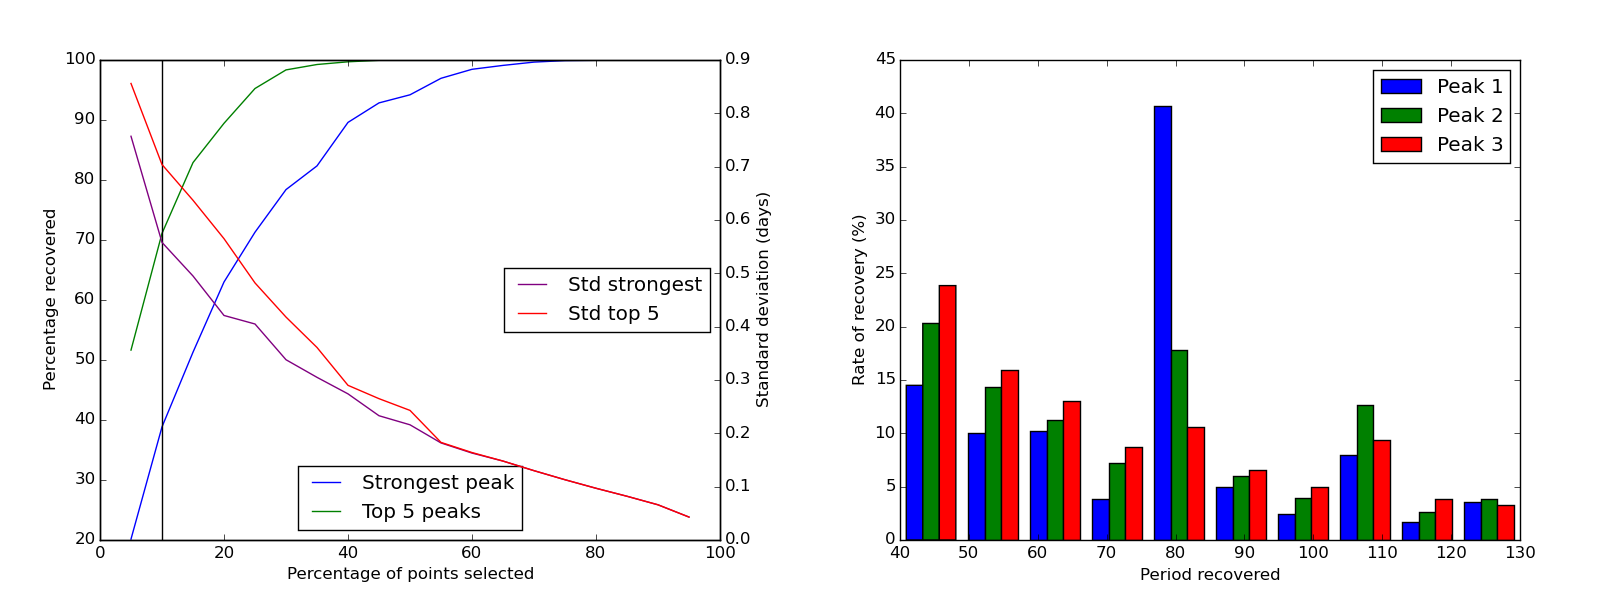
\includegraphics[scale=0.25]{Figures/prop.png} \\
\end{center}   
\caption{In this figure is illustrated the effects of randomly selecting a given proportion of the {\asas} data in terms
  of whether the same period of 82.6 days is recovered and the error in this result. The black vertical line shows
  approximately where the number of points in the {\harps} data would come. Also shown as the right panel is the
  distribution of the first 3 peaks in the periodograms returned when 10\% of the data is selected. The blue bar shows
  the distribution (as a percentage of the whole) of the strongest peak, the green the second strongest and the red the
  third strongest.}
\protect\label{fig:asasprop}
\end{figure}
